%%%%%%%%%%%%%%%%%%%%%%%%%%%%%%%%%%%%%%%%%%%%%%%%%%%%%%%%%%%%%%%%%%%%%%
%%  Copyright by Wenliang Du.                                       %%
%%  This work is licensed under the Creative Commons                %%
%%  Attribution-NonCommercial-ShareAlike 4.0 International License. %%
%%  To view a copy of this license, visit                           %%
%%  http://creativecommons.org/licenses/by-nc-sa/4.0/.              %%
%%%%%%%%%%%%%%%%%%%%%%%%%%%%%%%%%%%%%%%%%%%%%%%%%%%%%%%%%%%%%%%%%%%%%%

\documentclass[11pt]{article}

\usepackage[most]{tcolorbox}
\usepackage{times}
\usepackage{epsf}
\usepackage{epsfig}
\usepackage{amsmath, alltt, amssymb, xspace}
\usepackage{wrapfig}
\usepackage{fancyhdr}
\usepackage{url}
\usepackage{verbatim}
\usepackage{fancyvrb}
\usepackage{adjustbox}
\usepackage{listings}
\usepackage{color}
\usepackage{subfigure}
\usepackage{cite}
\usepackage{sidecap}
\usepackage{pifont}
\usepackage{mdframed}
\usepackage{textcomp}
\usepackage{enumitem}
\usepackage{ctex}


% Horizontal alignment
\topmargin      -0.50in  % distance to headers
\oddsidemargin  0.0in
\evensidemargin 0.0in
\textwidth      6.5in
\textheight     8.9in 

\newcommand{\todo}[1]{
\vspace{0.1in}
\fbox{\parbox{6in}{TODO: #1}}
\vspace{0.1in}
}


\newcommand{\unix}{{\tt Unix}\xspace}
\newcommand{\linux}{{\tt Linux}\xspace}
\newcommand{\minix}{{\tt Minix}\xspace}
\newcommand{\ubuntu}{{\tt Ubuntu}\xspace}
\newcommand{\setuid}{{\tt Set-UID}\xspace}
\newcommand{\openssl} {\texttt{openssl}}


\pagestyle{fancy}
\lhead{\bfseries SEED Labs}
\chead{}
\rhead{\small \thepage}
\lfoot{}
\cfoot{}
\rfoot{}


\definecolor{dkgreen}{rgb}{0,0.6,0}
\definecolor{gray}{rgb}{0.5,0.5,0.5}
\definecolor{mauve}{rgb}{0.58,0,0.82}
\definecolor{lightgray}{gray}{0.90}


\lstset{%
  frame=none,
  language=,
  backgroundcolor=\color{lightgray},
  aboveskip=3mm,
  belowskip=3mm,
  showstringspaces=false,
%  columns=flexible,
  basicstyle={\small\ttfamily},
  numbers=none,
  numberstyle=\tiny\color{gray},
  keywordstyle=\color{blue},
  commentstyle=\color{dkgreen},
  stringstyle=\color{mauve},
  breaklines=true,
  breakatwhitespace=true,
  tabsize=3,
  columns=fullflexible,
  keepspaces=true,
  escapeinside={(*@}{@*)}
}

\newcommand{\newnote}[1]{
\vspace{0.1in}
\noindent
\fbox{\parbox{1.0\textwidth}{\textbf{Note:} #1}}
%\vspace{0.1in}
}


%% Submission
\newcommand{\seedsubmission}{You need to submit a detailed lab report, with screenshots,
to describe what you have done and what you have observed.
You also need to provide explanation
to the observations that are interesting or surprising.
Please also list the important code snippets followed by
explanation. Simply attaching code without any explanation will not
receive credits.}

%% Book
\newcommand{\seedbook}{\textit{Computer \& Internet Security: A Hands-on Approach}, 2nd
Edition, by Wenliang Du. See details at \url{https://www.handsonsecurity.net}.}

%% Videos
\newcommand{\seedisvideo}{\textit{Internet Security: A Hands-on Approach},
by Wenliang Du. See details at \url{https://www.handsonsecurity.net/video.html}.}

\newcommand{\seedcsvideo}{\textit{Computer Security: A Hands-on Approach},
by Wenliang Du. See details at \url{https://www.handsonsecurity.net/video.html}.}

%% Lab Environment
\newcommand{\seedenvironment}{This lab has been tested on our pre-built
Ubuntu 16.04 VM, which can be downloaded from the SEED website.}






\newcommand{\seedlabcopyright}[1]{
\vspace{0.1in}
\fbox{\parbox{6in}{\small Copyright \copyright\ {#1}\ \ by Wenliang Du.\\
      This work is licensed under a Creative Commons
      Attribution-NonCommercial-ShareAlike 4.0 International License.
      If you remix, transform, or build upon the material, 
      this copyright notice must be left intact, or reproduced in a way that is reasonable to
      the medium in which the work is being re-published.}}
\vspace{0.1in}
}





\newcommand{\rebindingFigs}{./Figs}

\lhead{\bfseries SEED Labs -- DNS重绑定攻击实验}


\begin{document}

\begin{center}
{\LARGE DNS重绑定攻击实验}

\vspace{0.05in}
Updated on February 10, 2020
\end{center}

\seedlabcopyright{2019}


\newcounter{task}
\setcounter{task}{1}
\newcommand{\tasks} {\bf {\noindent (\arabic{task})} \addtocounter{task}{1} \,}



% *******************************************
% SECTION
% ******************************************* 
\section{实验介绍}


本实验的目的有两个:(1)演示DNS重绑定攻击的工作原理,以及(2)帮助学生获得有关
如何使用DNS重绑定技术攻击IoT设备的经验。在实验配置中,我们有一个模拟的IoT设备,
可以通过Web页面对其进行控制(许多IoT设备也是如此)。许多物联网设备没有强大的保护机制,
一旦攻击者可以直接与它交互,那么攻击者可以轻易地控制这些设备。


在本实验中模拟的IoT设备是一个恒温器,用于控制室内的温度。
要成功设置温度,客户端需要能与IoT服务器进行交互。由于IoT设备部署于防火墙之后,
因此外部计算机无法与IoT设备交互,因此无法控制恒温器。
为了突破防火墙的保护,攻击代码必须先进入内网,这一点并不困难。
每次用户从内网访问攻击者的Web站点时,攻击者的JavaScript代码就会在用户的浏览器中执行,
因此这个代码实际上是运行在内网中的。但是,由于浏览器实现了沙盒保护,所以即使攻击者的代码
位于内网中,也无法与IoT设备进行交互,


本实验的目的是使用DNS重绑定攻击来绕过沙盒保护,进而攻击者的JavaScript代码可以成功执行并从
IoT设备中获取必要的信息,然后利用这些信息将温度设置为一个非常高的值。本实验涵盖以下内容:


\begin{itemize}[noitemsep]
\item DNS服务器配置
\item DNS重绑定攻击
\item 对IoT设备进行攻击
\item 同源策略
\end{itemize}


\paragraph{相关阅读材料与视频:}
关于DNS协议与攻击的详细内容可以参考以下材料:

\begin{itemize}
\item Chapter 18 of the SEED Book, \seedbook
\item Section 7 of the SEED Lecture, \seedisvideo
\end{itemize}


\paragraph{Lab environment.} \seedenvironment



\vspace{0.2in}
\noindent
\fbox{\parbox{\textwidth}{
\noindent
\textbf{Customization.} 
在此次实验描述中,我们使用\texttt{attacker32.com}域作为攻击者控制的恶意域名。
当学生在进行本实验时,不被允许使用这个域名,学生应当使用一个包含自己名字的域名。
该要求的目的是区分学生的工作,由于该域名只在实验环境中可见,并不公开使用,因此任何域名
(即使已被他人拥有的域名)都可以在实验环境中安全地使用。
}}





% *******************************************
% SECTION
% ******************************************* 
\section{背景介绍: IoT}

我们的攻击目标是防火墙后面的一个物联网设备。我们并不能从外部直接访问这个物联网设备。
我们的目标是让内部用户运行我们的JavaScript代码,
这样我们就可以使用DNS重新绑定攻击与物联网设备交互。


许多物联网设备都有一个简单的内置web服务器,
这样用户可以通过web APIs与这些设备交互。
通常,这些物联网设备由防火墙保护,它们不能从外部直接访问。
由于这种类型的保护,许多物联网设备并没有实现强大的身份验证机制。
如果攻击者能够找到与它们交互的方法,就很容易危及其安全性。


我们使用一个简单的web服务器来模拟这种易受攻击的物联网设备,
该服务器提供两个API: \texttt{password}和\texttt{temperature},
物联网设备可以设置室温,为此,我们需要向服务器的\texttt{temperature} API发送一个HTTP请求;
其中请求应该包括两部分数据:目标温度值和密码。
密码是定期更改的,但可以使用\texttt{password}API获取。
因此,要想成功设置温度,用户首先需要获得密码,然后将密码附加到\texttt{temperature}API中发出。


这里的密码并不用于身份验证,它只是用于抵抗跨站请求伪造(CSRF)攻击。
如果没有这种保护,一个简单的CSRF攻击就足够了,没有必要使用复杂的DNS重新绑定攻击来实现目标。
为了简单起见,我们硬编码了密码,而在实际生产系统中,密码往往是定期重新生成的。



% *******************************************
% SECTION
% ******************************************* 
\section{实验环境搭建}

\begin{figure}[htb]
\centering
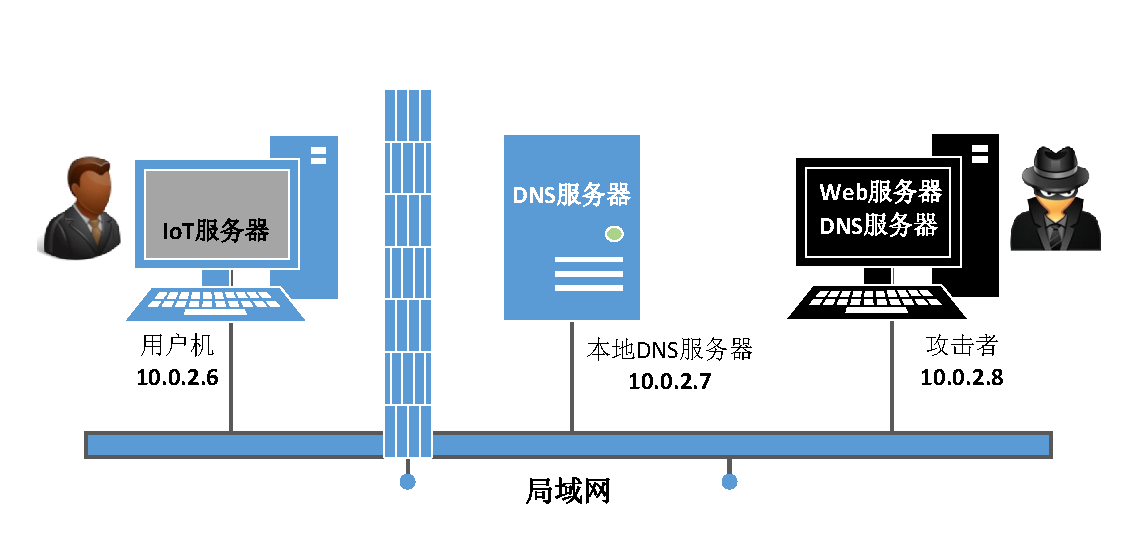
\includegraphics[width=0.9\textwidth]{\rebindingFigs/environment_setup_rebind.pdf}
\caption{实验环境搭建}
\label{dns:fig:rebind_environment}
\end{figure}


在本次实验中,我们将使用三台主机(VMs):用户主机、本地DNS服务器和攻击者主机。
为了简单起见,我们使用VirtualBox中的NAT网络适配器将这些虚拟机放在同一局域网中。
在真实环境中,它们并不会在同一局域网中。
我们还假设运行在用户主机上的IoT设备在防火墙后面,因此攻击者主机不能直接访问IoT设备。
这个实验环境的配置相当复杂,我们需要配置三个主机并在它们上运行多个服务器,
包括一个IoT web服务器(在用户主机上)、一个web服务器和一个DNS服务器(在攻击者主机上)
以及一个DNS服务器(在本地DNS服务器上)。因此我们将配置过程分为5个任务。


在之后的实验描述中,我们假设用户机的IP地址为{\tt 10.0.2.6},本地DNS服务器的IP地址为{\tt 10.0.2.7},
攻击者主机的IP地址为{\tt 10.0.2.8}。实验环境的拓扑
如图~\ref{dns:fig:rebind_environment}所示。



% -------------------------------------------
% SUBSECTION
% ------------------------------------------- 
\subsection{任务 1: 配置用户机}

\paragraph{Step 1. 降低Firefox的DNS缓存时间:}
为了减少DNS服务器的负载并加快响应时间,Firefox浏览器会缓存DNS结果。
默认情况下,这个缓存的过期时间为60秒。这也意味着我们的DNS重新绑定攻击需要等待至少60秒。
为了让我们的实验更轻松,我们把时间减少至10秒或更少。
在用户主机的Firefox中,在URL字段中输入\texttt{about:config}。
点击通过一个警告页面后,我们将看到一些首选项名称及其值的列表。
搜索\texttt{dnsCache},找到以下条目并修改它的值:


\begin{lstlisting}
(*@\textbf{network.dnsCacheExpiration}@*):  change its value to 10 (default is 60)
\end{lstlisting}

完成修改后,我们需要退出Firefox浏览器并重新启动它,否则修改不会生效。



\paragraph{Step 2. 修改\texttt{/etc/hosts}:}

我们需要将以下条目添加到/etc/hosts文件中。
我们将用\texttt{www.seeedIoT32.com}作为IoT的Web服务器域名。
此服务器可以运行在其他的主机上,但为了简单起见,
我们在用户主机上运行物联网服务器(其IP地址为\texttt{10.0.2.6}):


\begin{lstlisting}
10.0.2.6   www.seedIoT32.com
\end{lstlisting}
 


\paragraph{Step 3. 本地DNS服务器:}
我们需要配置用户主机以使用特定的本地DNS服务器。
这是通过将本地DNS服务器设置为解析器配置文件(\texttt{/etc/resolv.conf})中
的第一个\texttt{nameserver}条目来实现的。
有一个挑战是我们所提供的VMs都使用Dynamic Host Configuration Protocol(DHCP)来获取网络配置参数,
如IP地址、本地DNS服务器等。DHCP客户端将会用DHCP服务器提供的信息覆盖\texttt{/etc/resolv.conf}文件。

要将信息导入\texttt{/etc/resolv.conf}而不用担心DHCP,
一种方法是将以下条目添加到 \path{/etc/resolvconf/resolv.conf.d/head}文件
(假设\texttt{10.0.2.7}是本地DNS服务器的IP地址):


\begin{lstlisting}
nameserver 10.0.2.7
\end{lstlisting}

Head文件的内容将预先写入动态生成的解析器配置文件。
通常,这只是一个注释行(\texttt{/etc/resolv.conf}中的注释来自这个Head文件)。
在进行更改之后,我们需要运行以下命令使更改生效:

\begin{lstlisting}
$ sudo resolvconf -u
\end{lstlisting}


%----------------------------
\paragraph{Step 4. 测试:}
配置完用户主机之后,使用\texttt{dig}命令尝试获取一个主机名(hostname)的IP地址。
从dig的回显来查看响应内容是否是从本地的DNS服务器返回,如果不是则证明未成功配置。



% -------------------------------------------
% SUBSECTION
% ------------------------------------------- 
\subsection{任务 2: 在用户主机上开启IoT服务器}

在此任务中,我们将在用户主机启动IoT服务器。
通过web服务器,用户可以与IoT设备通信。


%-----------
\paragraph{Step 1. 安装Flask:}

我们使用\texttt{Flask}Web框架来开发IoT服务器。在当前版本的SEED VM中,\texttt{Flask}没有安装,
使用以下命令安装\texttt{Flask}。

\begin{lstlisting}
$ sudo pip3 install Flask==1.1.1
\end{lstlisting}


%-----------
\paragraph{Step 2. 开启IoT服务器:}
IoT服务器代码包含在\texttt{user\_vm.zip},可以从SEED Lab的网站上下载。
解压缩文件后,进入\texttt{user\_vm}文件夹,
运行写好的脚本\texttt{start\_iot.sh}或直接运行\texttt{"flask run"}来启动IoT服务器。
需要注意的是,我们使用端口\texttt{8080}作为IoT服务器
(该端口号在实验配置中是硬编码的,将其更改为不同的数字将破坏后续实验配置)。



\begin{lstlisting}
$ unzip user_vm.zip          # 解压缩文件
$ cd user_vm                 # 进入user_vm文件夹
$ FLASK_APP=rebind_iot flask run --host 0.0.0.0 --port 8080
\end{lstlisting}
 

%-----------
\paragraph{Step 3. 测试IoT服务器:}

要测试IoT服务器,请在用户主机的浏览器上访问以下URL。
如果一切都设置正确,我们应该能够看到一个恒温器,我们可以通过拖动滑动条来改变温度设置。
请在实验报告中给出屏幕截图。

\begin{lstlisting}
http://www.seedIoT32.com:8080
\end{lstlisting}



% -------------------------------------------
% SUBSECTION
% ------------------------------------------- 
\subsection{任务 3: 在攻击者主机上开启恶意Web服务器}

在本实验室,IoT设备只能从防火墙后进行访问,
即只有实验配置中的用户主机可以访问。
将恶意代码发送到用户主机上的一种典型方式是让用户访问我们部署的网站,
这样写在web页面上的JavaScript代码就可以进入用户主机上。
在此任务中,我们将启动一个web服务器来托管这些web页面。


%-----------
\paragraph{Step 1. 安装Flask:}

我们的恶意web服务器也是基于\texttt{Flask} web框架开发的,因此同样需要进行安装。


\begin{lstlisting}
$ sudo pip3 install Flask==1.1.1
\end{lstlisting}


%-----------
\paragraph{Step 2. 启动攻击者的Web服务器:}
攻击者的服务器代码包含在\texttt{attacker\_vm.zip}中,
可以从SEED Lab的网站上下载。解压缩文件后,进入\texttt{attacker\_vm}文件夹,
通过运行写好的脚本\texttt{start\_webserver.sh}或直接运行\texttt{"flask run"}来启动web服务器。



\begin{lstlisting}
$ unzip attacker_vm.zip      # 解压缩文件
$ cd attacker_vm             # 进入attacker_vm 文件夹
$ FLASK_APP=rebind_malware flask run --host 0.0.0.0 --port 8080
\end{lstlisting}



%-----------
\paragraph{Step 3. 测试攻击者的Web服务器:}
在攻击者主机的浏览器中输入以下URL,应该可以看到攻击者的Web站点。
请在实验报告中给出屏幕截图。



\begin{lstlisting}
http://localhost:8080
\end{lstlisting}


% -------------------------------------------
% SUBSECTION
% ------------------------------------------- 
\subsection{任务 4: 配置攻击者主机的DNS服务器}

攻击者主机也充当了\texttt{attacker32.com}域名的名称服务器。
BIND9服务器已经在攻击者主机上运行,我们要做的是为它准备一个区域文件。
区域文件的示例已在\texttt{attacker\_vm}文件夹中。
学生应该相应地更改区域文件,并将其复制到\texttt{/etc/bind}文件夹中
以下内容为区域文件的示例,第一个条目是响应包默认的Time-To-Live (\texttt{TTL})值(秒),
指明了收到的响应包会在DNS缓存中保存的时间。在后续的任务中,这个值可能需要修改。


\begin{lstlisting}
$TTL 10000
@       IN      SOA   ns.attacker32.com. admin.attacker32.com. (
                2008111001
                8H
                2H
                4W
                1D)

@       IN      NS    ns.attacker32.com.

@       IN      A     10.0.2.8
www     IN      A     10.0.2.8
ns      IN      A     10.0.2.8
*       IN      A     10.0.2.8
\end{lstlisting}
 

你需要在\texttt{/etc/bind/named.conf}中添加以下区域条目,这样上述的区域文件才会在
BIND9服务器中使用。


\begin{lstlisting}
zone "attacker32.com" {
        type master;
        file "/etc/bind/attacker32.com.zone";
};
\end{lstlisting}
 

完成修改\texttt{named.conf}文件后,我们需要用以下的命令来重启BIND9服务器。


\begin{lstlisting}
$ sudo service bind9 restart
\end{lstlisting}
 

\paragraph{测试:} 如果一切都设置正确,我们可以尝试以下\texttt{dig}命令,
看看我们得到的响应是否与我们在区域文件中配置的响应相同。请在实验报告中给出你的观察(截屏)。

\begin{lstlisting}
// 测试DNS服务器 (修改 10.0.2.8 为攻击者主机的IP)
$ dig @10.0.2.8 www.attacker32.com
\end{lstlisting}



% -------------------------------------------
% SUBSECTION
% ------------------------------------------- 
\subsection{任务 5: 配置本地DNS服务器}

在之前的任务中,我们已经配置了\texttt{attacker32.com}域(或学生自己选择的域名)的名称服务器。
为了让其他人可以找到这个名称服务器,我们需要在\texttt{.com}的名称服务器处注册我们的名称服务器,
这样会添加一条\texttt{NS}记录到它的数据库中。没有这个步骤,其他人的DNS请求无法到达我们的名称服务器。


为了实现这点,我们需要购买一个域名,并在一台公网主机上运行我们的名称服务器,而不是在内网中
运行一个虚拟机(我们的虚拟机是无法从外部进行访问的)。
尽管这些是可行的,但这大大提高了实验环境搭建的成本和复杂性。我们采用一种简单的方法来模拟真实的生产环境。


在本地DNSserver上,我们设置一个\texttt{attacker32.com}域的转发记录。
每当本地 DNS 服务器收到针对此域内主机的 DNS 查询时,
它会将 DNS 查询发送到转发记录中指定的 IP地址,
而不是前往根域名服务器和\texttt{.com}服务器去询问\texttt{attacker32.com}
域的名称服务器的地址。


要将此类记录添加到本地 DNS 服务器,我们需要将以下行添加到 \path{/etc/bind/named.conf}
(值得注意的是,学生应该使用他们自己定制的域名,而不是使用\texttt{attacker32.com})。


\begin{lstlisting}
zone "attacker32.com" {
    type forward;
    forwarders { 10.0.2.8; };
};
\end{lstlisting}

如果你从PDF文件复制并粘贴以上内容,请当心引号的格式可能不正确,这会导致配置文件的错误。
可以选择删除它们,并手工输入引号。在配置完BIND9后,我们需要运行以下命令来重启DNS服务器:


\begin{lstlisting}
$ sudo service bind9 restart
\end{lstlisting}

%Check the BIND9's log file at \texttt{/var/log/syslog} to
%see whether there is any error message. 


\paragraph{测试:}
如果我们正确完成了任务1-5,当我们在用户主机运行\texttt{dig}命令来查找任何 \texttt{attacker32.com}
域下的子域名的IP地址时,我们应该得到攻击者主机在\texttt{attacker32.com}区域文件中配置的值。


\begin{lstlisting}
$ dig xyz.attacker32.com
\end{lstlisting}
 


请在实验报告中给出你的观察(截屏)。如果没有得到IP地址,可能是在某一个步骤做错了。
你应该先修复它,然后再进行下一个任务。




% *******************************************
% SECTION
% ******************************************* 
\section{针对IoT设备进行攻击}

我们已经做好了攻击IoT设备的准备,为帮助学生更好地理解攻击的原理,
我们将攻击拆分为以下几个递进的步骤。


\subsection{任务 6. 理解同源策略防护}

在此任务中,我们将做一些实验来理解浏览器实现的同源策略保护。在用户主机上,我们
访问以下三个URLs。最好是在三个不同的Firefox窗口打开这三个页面(而不是同一个窗口的三个tab),
这样他们都是可见的。


\begin{lstlisting}
URL 1:  http://www.seedIoT32.com:8080
URL 2:  http://www.seedIoT32.com:8080/change
URL 3:  http://www.attacker32.com:8080/change
\end{lstlisting}


第一个页面让我们看到了当前恒温器设定的温度(见图~\ref{rebinding:fig:webpages}.a);
它每秒从IoT服务器获取当前的温度值。我们需要让这个页面保持打开的状态,这样我们可以时刻观察到
恒温器当前的温度设定。
第二第三个页面看上去是相同的(见图~\ref{rebinding:fig:webpages}.b),除了前者从IoT服务器来,
后者从攻击者服务器来。当我们在这两个页面中点击按钮,它们会向IoT服务器发出一个设定温度的请求。
我们希望将恒温器的温度提高到\texttt{99}摄氏度。



\begin{figure}[htb]
\begin{center}
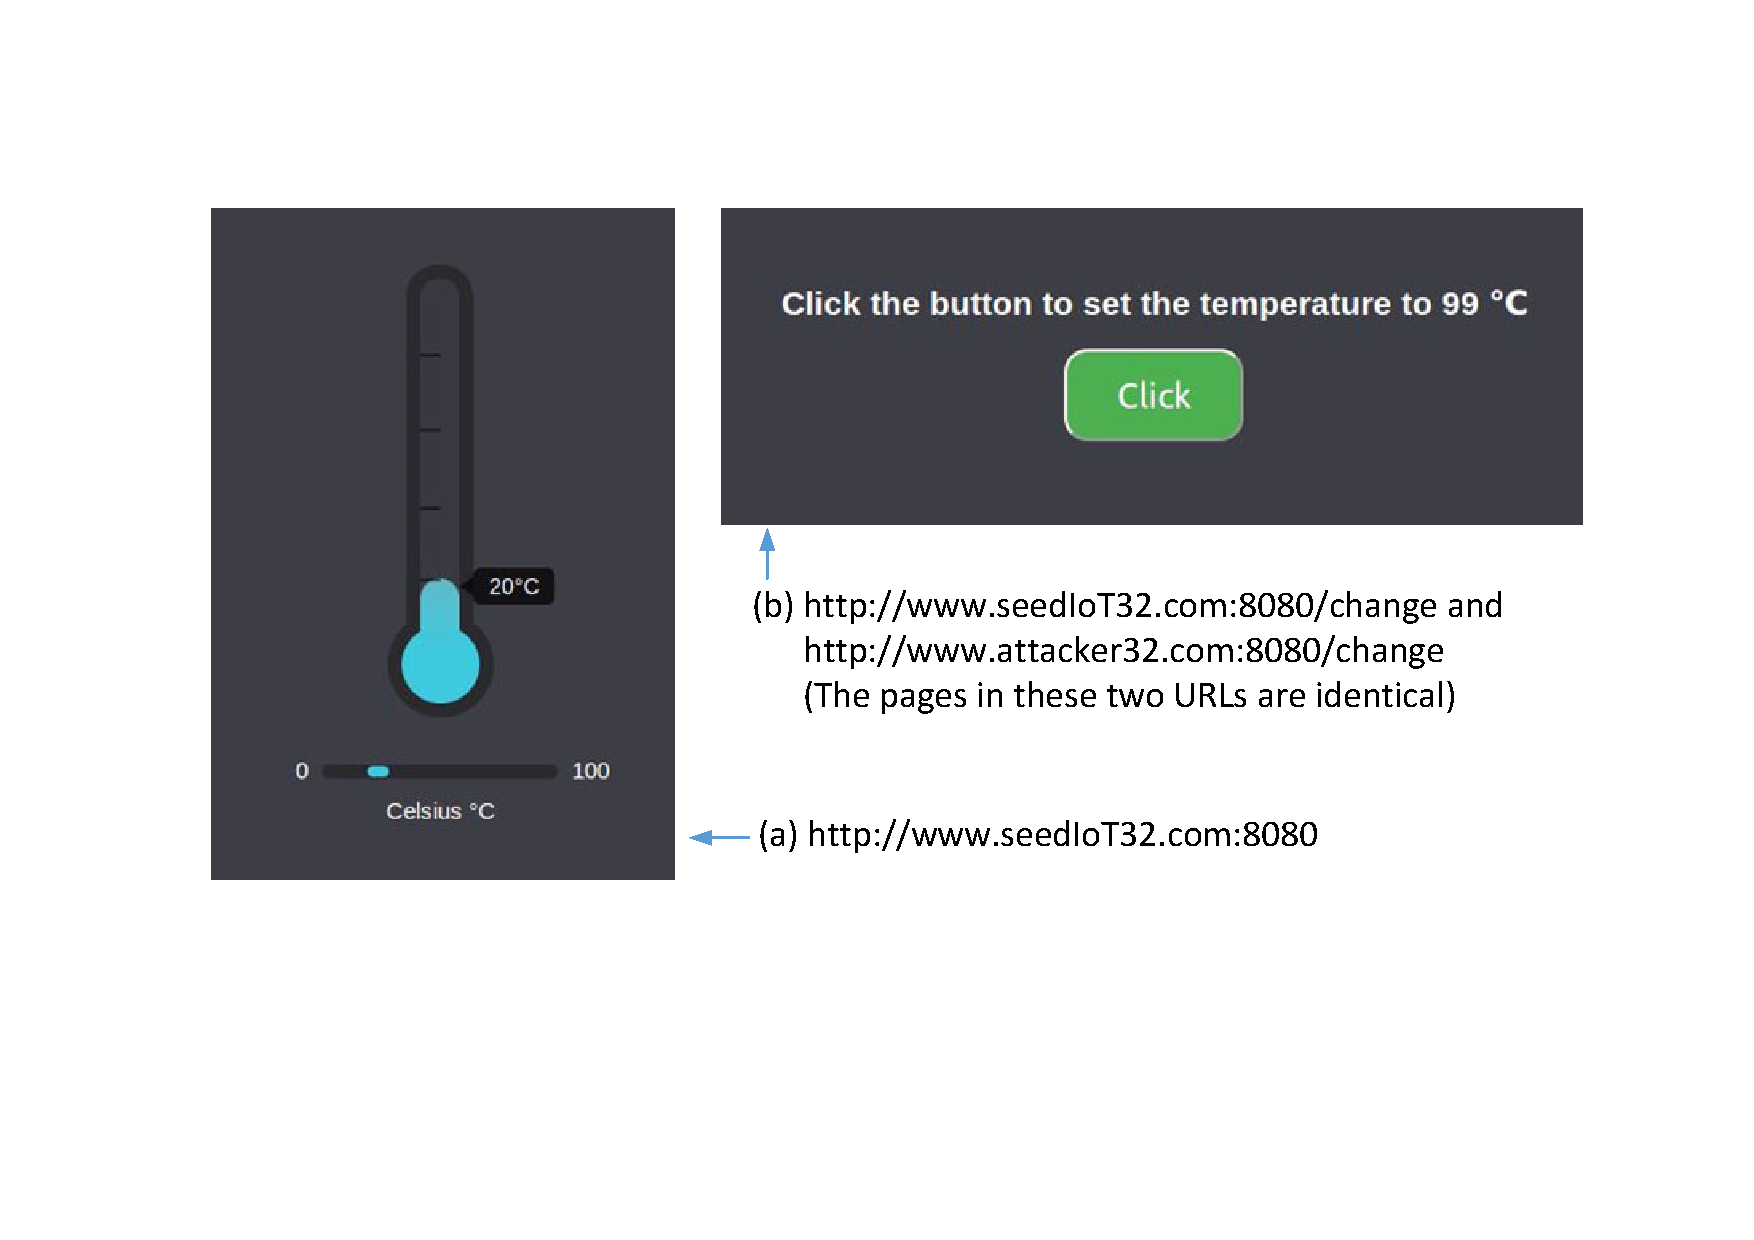
\includegraphics[width=0.8\textwidth]{\rebindingFigs/iot_webpages.pdf}
\end{center}
\caption{从三个URLs获取的Web页面}
\label{rebinding:fig:webpages}
\end{figure}
 

点击第二第三个页面中的按钮,并描述你的观察。哪个可以成功设置恒温器的温度?请解释为什么。
要找到原因,请在Firefox中点击以下菜单序列。这将出现一个控制台窗口,查看错误信息(如果有)。
提示:出错原因与浏览器实行的同源策略有关。请解释为什么这个策略导致其中一个页面失败了。

\begin{lstlisting}
Tools -> Web Developer -> Web Console
\end{lstlisting}
  



% -------------------------------------------
% SUBSECTION
% ------------------------------------------- 
\subsection{任务 7. 绕过同源策略防护}


从之前的任务来看,由于浏览器的同源策略保护,似乎不可能从攻击者页面设定恒温器的温度。
此任务的目标是绕过这个保护,让我们可以从这个页面设置恒温器的温度。


绕过同源策略防护的主要想法基于这样一个事实:策略的执行是基于主机名,而不是IP地址,
所以只要我们使用\texttt{www.attacker32.com}的URL,我们遵守SOP的策略,但这
并不意味着我们被限制与\texttt{www.attacker32.com}的Web服务器通信。


在用户浏览器向\texttt{www.attacker32.com}发送请求之前,它首先需要知道\texttt{www.attacker32.com}的
IP地址。所以用户主机会发出一个DNS请求,如果IP地址没有在本地DNS服务器里缓存,那么DNS请求最终会
被发送到\texttt{www.attacker32.com}的名称服务器,即攻击者主机。
因此,攻击者可以在这个响应中放入任何信息。



\paragraph{Step 1: 修改JavaScript代码:}
在攻击者主机中,\url{www.attacker32.com:8080/change}运行的JavaScript代码位于文件:
\path{attacker_vm/rebind_malware/templates/js/change.js}中。由于该页面来自\texttt{www.attacker32.com}
服务器,根据同源策略,它只能与同一服务器交互。因此我们将代码的第一行从\url{http://www.seediot32.com:8080} 
改为以下内容:

\begin{lstlisting}
let url_prefix = 'http://www.attacker32.com:8080'
\end{lstlisting}
 

完成修改之后,重启攻击者主机的Web服务,接着在用户主机上刷新页面,重新点击按钮。
还能看到控制台的错误信息吗?请解释你观察到的现象。




\paragraph{Step 2: 进行DNS重绑定:}
我们的JavaScript代码发送请求到\url{www.attacker32.com},
请求将返回到攻击者主机。但这不是我们想要的,我们希望将请求发送到IoT服务器。
这一点可以通过DNS重绑定技术实现。
我们首先映射\url{www.attacker32.com}为攻击者主机的IP地址,
这样用户可以从\url{http://www.attacker32.com/change}打开攻击页面。
在我们点击网页上的按钮之前,我们重新映射\url{www.attacker32.com}主机名
到IoT服务器的IP地址,所以当点击按钮时,触发的请求将到达IoT服务器。这正是我们想要的攻击效果。


为了修改DNS映射,学生可以修改
\path{attacker32.com.zone}文件。完成修改之后,重启BIND9服务来重新加载区域内容。


\begin{lstlisting}
$ sudo rndc reload attacker32.com
\end{lstlisting}
 

如果此任务的两个步骤都正确完成,从\url{www.attacker32.com}的页面点击\texttt{change}按钮,
恒温器的温度将被成功设置。请在实验报告中给出攻击成功的证据(截屏)。



% -------------------------------------------
% SUBSECTION
% ------------------------------------------- 
\subsection{任务 8. 实施攻击}

在之前的任务中,用户必须点击按钮来将恒温器设置到一个很高的温度。显然,对于用户来说不太可能
去做这个。在此任务中,我们将自动完成这一操作。我们创建了一个Web页面来实现这一目的,
可以通过以下URL进行访问:



\begin{lstlisting}
http://www.attacker32.com:8080
\end{lstlisting}
 

一旦你在用户主机中加载这一页面,你会看到一个计时器正在从10倒数到0。
一旦计时器到达0,JavaScript代码会向\url{http://www.attacker32.com:8080}发出一个设置温度的请求,
并重新将计时器的计数复位到10。学生需要使用DNS重绑定技术,使得当计时器到达0时,
恒温器的温度会被成功改变。




% *******************************************
% SECTION
% *******************************************
\section{Submission}

\seedsubmission


\end{document}
